\chapter{Background}
% affine transformation
% image alignment
%features in the images
% machine learning
% nn and cnn
% transfor learning 
% computer vision
In computer vision\cite{forsyth2002computer}, there are existing solutions to find the affine transformations\cite{mikolajczyk2004scale} between two images, mainly by using SIFT\cite{lowe2004distinctive} and RANSAC\cite{fischler1981random}. This work will focus on by using machine learning idea to do the job. This chapter will provide a background introduction to machine learning, including supervised learning, unsupervised learning. Also, the process of image alignment by using both SIFT RANSAC and machine learning.
\section{Machine Learning}
In this work we using the supervised learning to approach this problem. In supervised learning, every training data are associated with labels, in our case, the label is the affine transformation, and the data will be the images. In this section, we will provide the general description of neural network and convolutional neural network, which both are using in the model.

\section{Affine transformation}
Affine transformation\cite{svoboda2007image} take three pairs of corresponding points, which is sufficient to find the coefficients. The affine transformation includes typical geometric transformations such as rotation, translation and skewing. Affine transformation has the following properties, origin does not necessarily map to origin, lines map to line, parallel lines remain parallel after the transformation and ratios are preserved. For the translation matrix 
$\begin{pmatrix}
1&0&tx \\
0&1&ty \\
0&)&1
\end{pmatrix}$
will translate the image by $tx$ horizontally and $ty$ vertically and the rotation matrix 
$\begin{pmatrix}
\sin(\theta)&-\sin(\theta)&0 \\
\sin(\theta)&\cos(\theta)&0 \\
0&0&1
\end{pmatrix}$ will rotate the the image by $\theta$, we can take the product of the translation matrix and rotation matrix that can translate and rotate the image. 

\subsection{Neural network}
Neural networks are a popular architecture in machine learning, mainly involving input layer, hidden layers, and output layers. Each layer of a network consists of one or more neurons, each of which is connected with a weighting factor $w_{io}$ to all of the input $i$. In the simple case, the network has two inputs, as sketched in figure 2.1. 
\begin{figure}
  \centering
    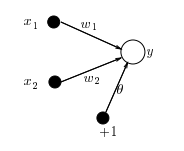
\includegraphics[width=3.0in]{figs/nn_2.1}
    \caption{Single layer network with one output and two inputs\cite{krose1993introduction}}
\end{figure}
The input of the neuron is the weighted sum of the inputs plus the bias term. The output of the network is formed by activation of the output neuron, which is some function of the inputs. 
\begin{align*}
F(y) &=  \sum_{i=1}^{2}w_ix_i+\theta
\end{align*}
There are many activation functions that we can choose, but in this work, we are mainly using the rectified linear unit, $ReLu$, a non-linear function shown in Figure 2.2.
\begin{figure}
\centering
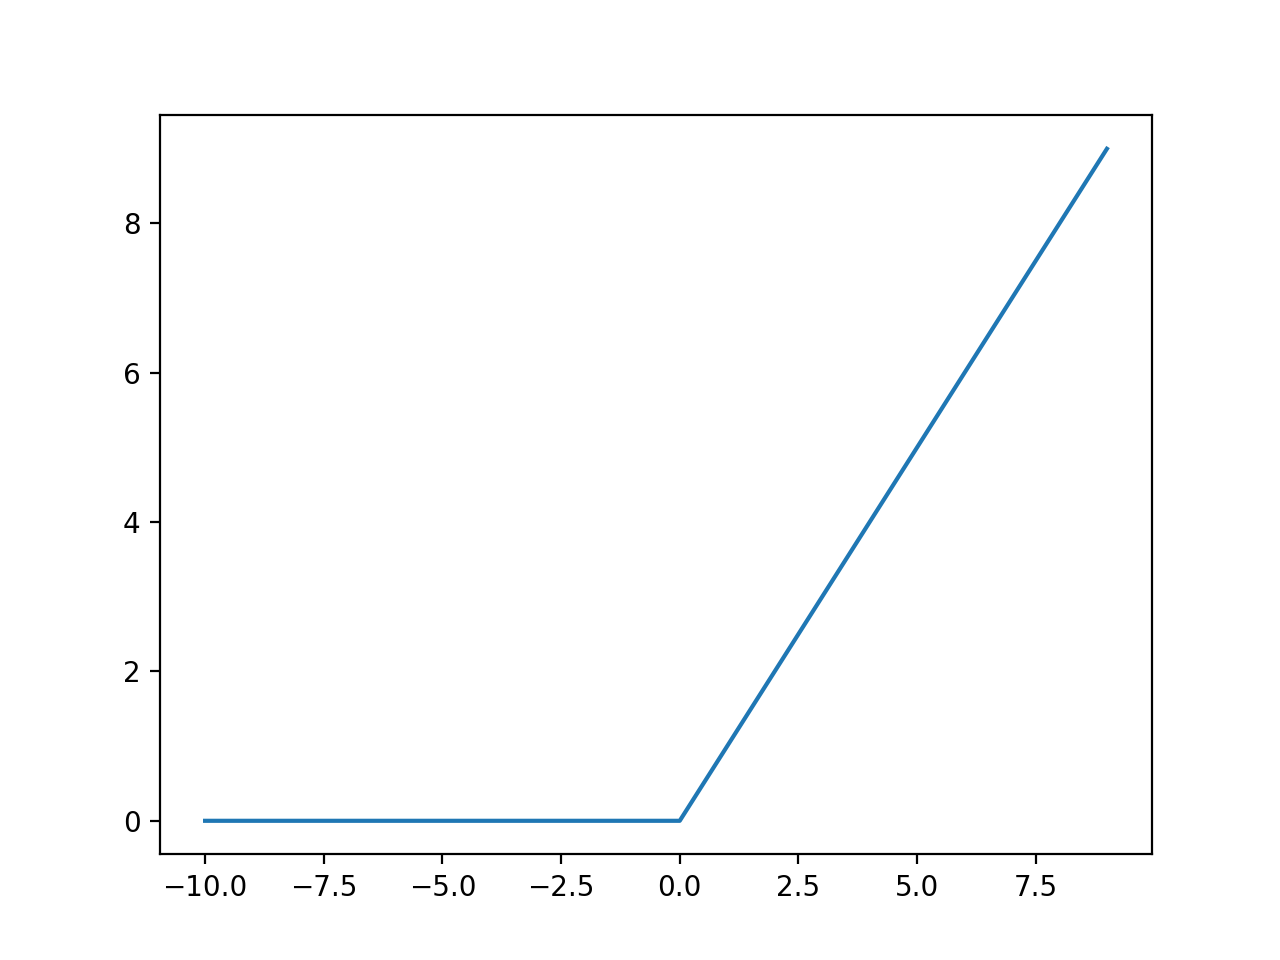
\includegraphics[width=3.0in]{figs/relu}
\caption{The Rectified Linear Unit (ReLU) activation function\cite{nair2010proceedings}}
\end{figure}
When training a network, there is two steps in training, which is forward-propagation and back-propagation. When doing forward-propagation each layer consists of units which receive their inputs from a layer directly below and send their output to units in a layer directly above the unit after the activation function. Their are no connection within a layer. After we will have some way to measure the error from the outputs, also know as $ cost\ function$. In this work we are using mean square error to measure the differences between the network prediction and the ground truth which is the parameters of affine transformation matrix in our case. After measuring the 'error', the network performs a back-propagation to adjust the weight. The trick is to apply the chain rule to find the partial derivative of the neurons. The goal of the neural network is to minimize the cost function. This is a basic neural network, also called fully connected neural network\cite{krose1993introduction}. 

\subsection{CNN(Convolutional Neural Network)}
  A convolutional neural network (CNN) is known to be good when dealing with image tasks. In this work, we are dealing with aerial photography. Using the CNN\cite{lecun1989backpropagation} is known to be efficient to dealing with image processing tasks\cite{goodfellow2016deep}. The Convolutional neural network includes a few basic concepts. First, there is a filter matrix, the purpose of the filter matrix is to detect the features in the images, and different filters may detect different features in the images.
Features can be considered like the interesting points in an image. These can include 
\begin{itemize}
\item corners where horizontal and vertical lines may meet
\item horizontal features like horizon lines
\item vertical features like edges of vertically oriented fields
\end{itemize}
Figure 2.3 shows horizontal and vertical features in an example image. When we apply the filter matrix to an image, the outcome of the image may shrink, one way to avoid this problem is applying padding to the image. There are two different types of padding, same padding or valid  padding, we can get the same size of output image after filtering by using same padding, or we can use valid padding and the size of the output image after filtering will be different than the original image. 
 
Also there is a term call 'stride' in CNN models. Stride refers to how many pixels the filter moves each time it is applied. For example if the stride is 1, then the filter is applied on every pixel. A filter starts in the upper left corner of an image. \\
\begin{figure}
  \centering
    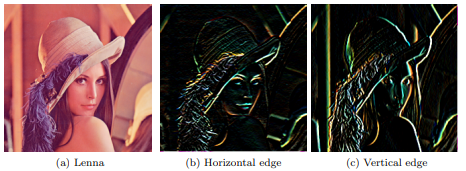
\includegraphics[width=4.0in]{figs/cnn_hv_features}
    \caption{Example image with horizontal and vertical features shown.\cite{wu2017introduction}}
\end{figure}
The convolutional layer is where the data transformation takes place. It includes many filters so that it can detect different features in the input images. After applying a convolution layer typically we apply a pooling layer. There are max pooling or average pooling, max pooling is an operation that calculates and extracts the max value in each patch of each feature map. On the other hand, average pooling operation that calculates and extracts the average value in each patch of each feature map\cite{wu2017introduction}.\\
After many repetitions of convolutional and pooling layers, we will have the fully connected layer that vectorizes all the features from the last pooling layer. This is also called a fully connected layer. \\
In the last layer, we have our loss layer, it act differently based on the loss function that we implement. Suppose $y_1$ is the corresponding label value for input $x_1$, the loss function can be used to measure how wrong is the CNN prediction $y_p$ and the $y_1$. Figure 2.4 shows the general architecture of a CNN model.



\begin{figure}
  \centering
    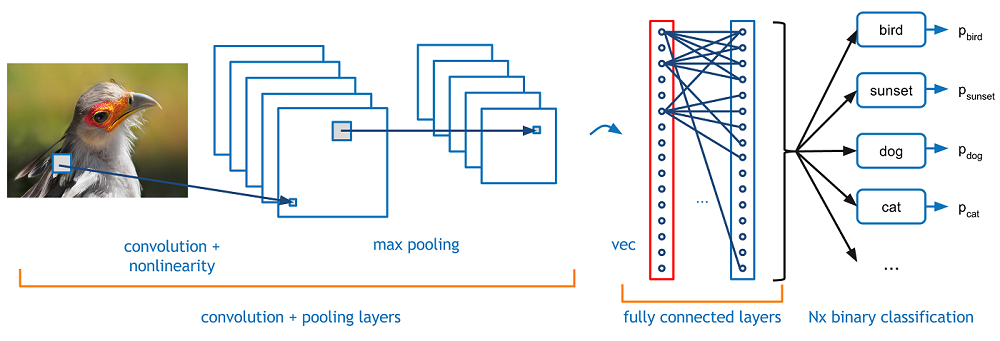
\includegraphics[width=4.5in]{figs/cnn_arch}
    \caption{The architecture of a CNN\cite{cnn}}
\end{figure}

\subsection{Transfer learning}
Transfer learning\cite{pratt1997second} can be very useful with certain machine learning or data mining model. Transfer learning allows us to use the knowledge within a neural network that has already been trained and apply that knowledge to help solve a new task. That means we can find a neural network that is has been trained to do some task, and we strip of the last few layers in the pre-trained neural network and add own customized layers after that, so that when we train the neural network we only need to train the new layers that we added while retaining the knowledge of the other layers.\\
The problem of building and training a model from scratch is that sometimes it is too hard or is impossible to collect enough data for the model, or it takes too much resources to train and build the model from scratch. By using transfer learning, we may avoid these expenses. Transfer learning can be applied to different machine learning problems like regression, classification or clustering.\\
In transfer learning, we find a pre-trained machine learning model and we only keep the part that we need to keep in the model, and we add some new layers after. We only need to train the layers that come after the original model, which can save data and time. Figure 2.5 shows briefly how transfer learning works.

\begin{figure}
  \centering
    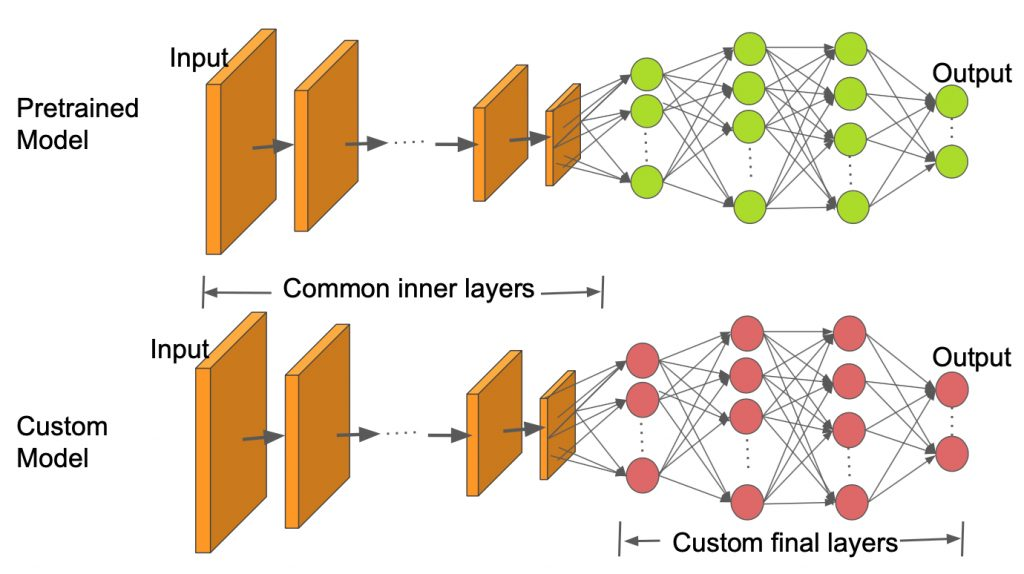
\includegraphics[width=3.0in]{figs/transfer_learning}
    \caption{A pre-trained model (above) has the last layers (green) removed and replaced so that the model may be reused for a new task (below). This process is called Transfer Learning.\citep{TL}}
\end{figure}


\section{SIFT and RANSAC}

One of the traditional solution for finding an affine transformation between two images is by using SIFT and RANSAC algorithms. The Scale Invariant Feature Transform(SIFT) is capable of finding the interesting features in a image even if the image is scaled or rotated. \cite{lowe1999object}\\
\begin{figure}
	\centering
	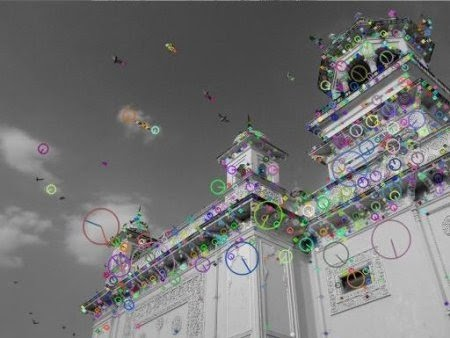
\includegraphics[width=3.0in]{figs/sift}
    \caption{Example of the SIFT algorithm finding interest points (features) in an image.\cite{sift_cv}}
\end{figure}

The Random Sample Consensus(RANSAC) estimates the parameters of a model by random sample of observed data and comes up with the best parameters that fit most of the data. After we have the found correspondences between features in two images we can generate the transformation matrix to align those two pictures.
\begin{figure}
	\centering
	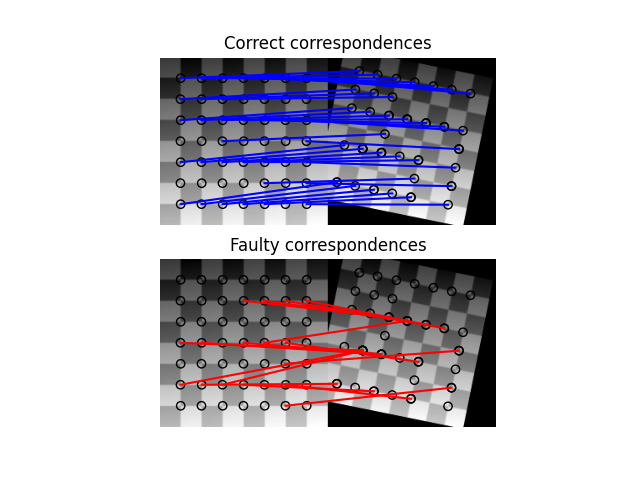
\includegraphics[width=3.0in]{figs/ransac_correct}
    \caption{Example of the RANSAC algorithm finding correspondences between two images.\cite{ransac_ski}}
\end{figure}

\section{Image Alignment}
This section will provide a high level introduction to image alignment and stitching. Image alignment involves many algorithms that work together so that the computer can align multiple images and stitch them together. Image alignment involves:
\begin{itemize}
\item finding common features between two images
\item matching the common features
\item generating the transformation between the images so that we can align them together.
\end{itemize}
 
For given two images, the first step is to find the common features between those images. Traditionally this may be done using SIFT \cite{lowe2004distinctive}. SIFT became a popular tool for finding common features in images between it is robust to handle images that vary in orientation, zoom and illumination. In simple terms SIFT can handle rotations, shifts and different colors in images.\\
Second, after we have found features in the images we need to find which features in one image match to which features in the other image. We can use RANSAC\cite{fischler1981random} for this goal. RANSAC will allow us to estimate the image transformation parameters that will align a number of features in one image with a set of features in another image. The following indented section follows from Brown and Lowe \cite{brown2007automatic} in their paper that outlines who to perform image stitching using RANSAC.\\
\begin{quote}
We denote the features that overlap in an image as $n_f$ and number of inlier $ n_i$. The trial result of image matching has one of two outcomes: $ m \in \{0,1\}$, and also for each trial for the feature matching $f^(i) \in \{0,1\}$ also only has binary outcomes, we assume it to be independent Bernoulli, so the number of inliers can be fit into Binomial distribution:\\
\begin{align*}
	p(f^{1:n_f} | m=1) = B(n_i;n_f,p1)\\
	p(f^{1:n_f} | m=0) = B(n_i;n_f,p0)
\end{align*}
Where the Binomial distribution is define as below:
\begin{align*}
	B(x;n, p) = \binom{n}{x} \cdot p^x(1-p)^{n-x}
\end{align*}
We can choose the value of $p_1 =0.6$ and value of $p_0 =0.1$, and we can applying  Bayes' Rule to find out if the images are matching:
\begin{align*}
p(m=1|f^{1:n_f}) = \frac{p(f^{1:n_f} | m=1) \cdot p(m=1)}{p(f^{1:n_f})}
\end{align*}
that give us the probability of if the image is matching base on the probability of the feature matching in the image. In Figure 2.8, shows the outcome of an image alignment and stitching example using aerial photographs.
\end{quote}



   

\begin{figure}
  \centering
    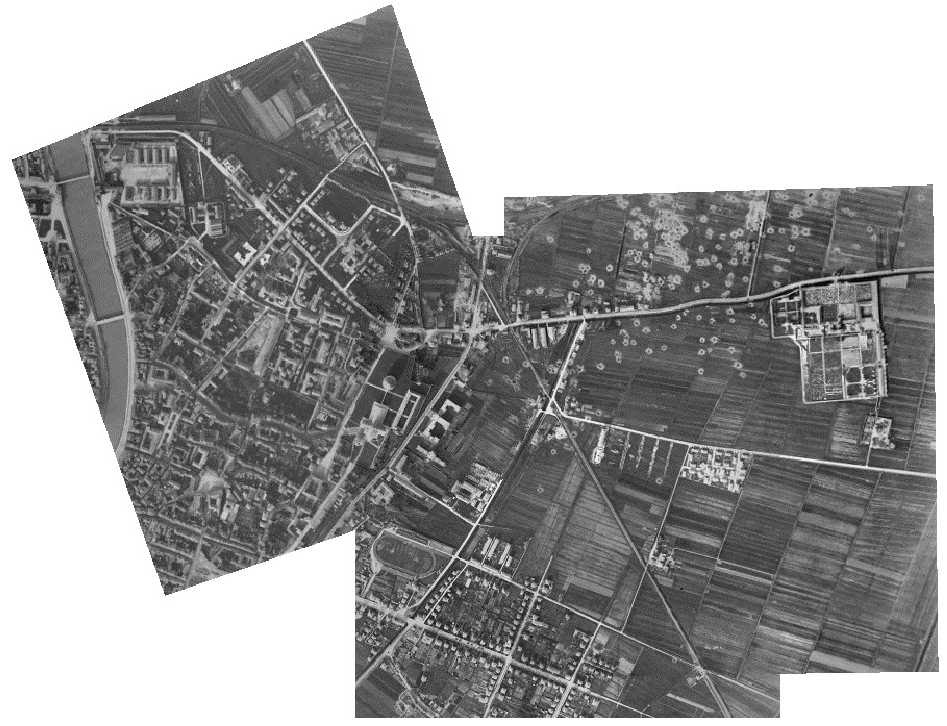
\includegraphics[width=3.0in]{figs/img_alignment}
    \caption{Aerial image alignment and stitching from three aerial photographs containing overlapping data.}
\end{figure}


